\documentclass{article}
\usepackage{indentfirst}
\usepackage{graphicx} % Required for inserting images
\graphicspath{{figure/}}
\usepackage{fullpage}
\usepackage{float}
\usepackage{amsmath}
\usepackage{xcolor}
\usepackage{subcaption}
\usepackage{tikz}
\usetikzlibrary{positioning}

\usepackage{cleveref}
\crefname{figure}{Fig.}{Figs.}
\Crefname{figure}{Fig.}{Figs.}
\crefname{table}{Table.}{Tables.}
\Crefname{table}{Table.}{Tables.}



\title{\textbf{Two steam instability - Numerical Physics project}}
\author{Qien Jing, Han Zhao}
\date{December 2025}

 
\begin{document}

\maketitle

\section{Introduction}
The two stream instability is a fundamental collective phenomenon in plasma physics and serves as a canonical model for studying the self-consistent interaction between charged particles and electrostatic fields. It captures key kinetic processes such as wave particle interaction and nonlinear trapping. Because these mechanisms arise from the detailed structure of the velocity distribution function $f(v)$, rather than fluid moments like the average velocity, they lie beyond the capability of magnetohydrodynamic (MHD) models, which assume a single bulk velocity and an approximately Maxwellian distribution at all times. When forward-accelerated electrons encounter decelerated ones, two distinct velocity streams may coexist, making fluid descriptions inadequate.

A fully kinetic treatment is therefore required. Solving the Vlasov equation is ideal but computationally demanding, whereas the Particle-in-Cell (PIC) method provides a practical alternative: it evolves particle trajectories and electromagnetic fields self-consistently at considerably lower cost. Widely used across plasma physics, astrophysics, and accelerator science, PIC combines a Lagrangian representation of charged particles with an Eulerian field solver. Its core cycle consists of charge deposition, field solving, field gathering, and particle pushing.

In this work, we focus on a simplified \textbf{1D3V electrostatic PIC system}, where the spatial domain is one-dimensional with periodic boundaries while particles retain three velocity components. Only the longitudinal electric field $E_x$ is solved from Poisson's equation; transverse fields and magnetic fields are included as placeholders for future extension to a full electromagnetic PIC model.

Electrons are initialized in a two beam configuration with opposite beam velocities, exciting the classical two stream instability. The objective of this report is to describe the code implementation, validate its linear growth rates against theory, and analyze nonlinear saturation and the resulting phase space structures. To support future extensions, we developed a fully functional and modular 1D3V electrostatic PIC code.


\section{Two stream Instability: Fluid Theory}

In order to interpret the results obtained from the PIC simulation, it is useful
to derive the theoretical dispersion relation of the cold two stream instability.
Under the cold-plasma approximation, the electron distribution function collapses into a Dirac delta function, which implies that the Vlasov equation becomes equivalent to its lower-order moment equations (the fluid equations). In this regime, the dispersion relation of the two stream instability can be derived directly from the fluid formulation.

We consider a one-dimensional electrostatic system consisting of two cold electron
beams propagating in opposite directions with beam velocities $+v_{0}$ and $-v_{0}$.
The ions form a fixed neutralizing background ($n_{i1}=0$).  Each electron beam has
density $n_{0}/2$, so that the total electron plasma frequency is
\[
\omega_{p}^{2}=\frac{n_{0}e^{2}}{\varepsilon_{0}m}.
\]

\subsection{Linearized fluid equations}

For each electron beam ($j=1,2$), the continuity and momentum equations are
\begin{align}
\frac{\partial n_{j}}{\partial t}+\nabla\!\cdot(n_{j}v_{j})&=0, \\
m\frac{\partial v_{j}}{\partial t} &= -eE .
\end{align}
We linearize around the equilibrium
\[
n_{j}=n_{0j}+n_{1j},\qquad 
v_{j}=v_{0j}+v_{1j},
\]
with
\[
n_{01}=n_{02}=\frac{n_{0}}{2},\qquad 
v_{01}=+v_{0},\quad v_{02}=-v_{0}.
\]

Assuming perturbations of the form
\[
E_{1}=E\,e^{i(kx-\omega t)},
\]
the linearized equations become
\begin{align}
-i(\omega-kv_{0j})\,n_{1j}+ik\,n_{0j}v_{1j}&=0,  \\
-i(\omega-kv_{0j})\,m\,v_{1j}&=-eE .
\end{align}
Solving for $v_{1j}$ and $n_{1j}$ yields
\begin{align}
v_{1j}&=\frac{eE}{m(\omega-kv_{0j})}, \\
n_{1j}&=\frac{e k n_{0j}}{m}\frac{E}{(\omega-kv_{0j})^{2}} .
\end{align}


The Poisson equation in Fourier space is
\[
ikE=\frac{\rho_{1}}{\varepsilon_{0}}
     =-\frac{e}{\varepsilon_{0}}(n_{11}+n_{12}),
\]
where ions do not contribute ($n_{i1}=0$).  
Substituting the density perturbations gives
\[
1=\sum_{j=1}^{2}\frac{n_{0j}e^{2}}{\varepsilon_{0}m}
   \frac{1}{(\omega-kv_{0j})^{2}}
  =\sum_{j=1}^{2}\frac{\omega_{pj}^{2}}{(\omega-kv_{0j})^{2}},
\]
with $\omega_{pj}^{2}=n_{0j}e^{2}/(\varepsilon_{0}m)$.

For the symmetric two-beam system,
\[
\omega_{p1}^{2}=\omega_{p2}^{2}=\omega_{p,beam}^{2}=\frac{\omega_{p}^{2}}{2},
\qquad 
v_{01}=+v_{0},\ v_{02}=-v_{0},
\]
so the dispersion relation becomes
\begin{equation}
1=\omega_{p,beam}^{2}
   \left[
   \frac{1}{(\omega-kv_{0})^{2}}
   +\frac{1}{(\omega+kv_{0})^{2}}
   \right].
\label{eq:twostream-dispersion}
\end{equation}

% \subsection{Dimensionless form}

% Introducing the normalizations
% \[
% x=\frac{\omega}{\omega_{p}},\qquad 
% y=\frac{k v_{0}}{\omega_{p}},
% \]
% we obtain the compact dimensionless form
% \begin{equation}
% \boxed{
% 1 = F(x,y)
%   = \frac{1}{2}
%     \left[
%     \frac{1}{(x-y)^{2}}
%     +\frac{1}{(x+y)^{2}}
%     \right].
% }
% \label{eq:dimensionless}
% \end{equation}

\subsection{Most unstable mode and growth rate}

To determine the most unstable mode of the symmetric cold two stream instability,
we start from the cold-fluid dispersion relation for two counter-propagating beams of
velocity $\pm v_0$,
\begin{equation}
    1 - \frac{\omega_{p}^2}{(\omega - kv_0)^2}
      - \frac{\omega_{p}^2}{(\omega + kv_0)^2} = 0.
\end{equation}

Expanding the denominators and collecting terms gives a quartic equation in $\omega$,
\begin{equation}
    \omega^4 - 2\omega^2 (k^2 v_0^2 + \omega_p^2)
    + k^4 v_0^4 - 2 k^2 v_0^2 \omega_p^2 = 0.
\end{equation}
Let $X=\omega^2$, so that the dispersion relation becomes a quadratic equation,
\begin{equation}
    X^2 - 2(k^2 v_0^2 + \omega_p^2)X
    + k^4 v_0^4 - 2k^2 v_0^2 \omega_p^2 = 0 .
\end{equation}

The unstable branch is the one with $X=\omega^2<0$. Solving the quadratic gives
\begin{equation}
    \omega^2 = k^2 v_0^2 + \omega_p^2
    - \omega_p \sqrt{4k^2 v_0^2 + \omega_p^2}.
\end{equation}
Inside the unstable region $\omega = i\gamma$, therefore
\begin{equation}
    \gamma^2
    = \omega_p \sqrt{4k^2 v_0^2 + \omega_p^2}
      - (k^2 v_0^2 + \omega_p^2).
\end{equation}

Define a dimensionless parameter $a \equiv k v_0/\omega_p$, which yields the normalized growth rate
\begin{equation}
    \frac{\gamma^2}{\omega_p^2}
    = \sqrt{4 a^2 + 1} - (a^2 + 1)
    \equiv f(a).
\end{equation}

The most unstable mode satisfies $\frac{df}{da}=0$, thus the wavenumber of the most unstable mode is
\begin{equation}
    a = \frac{\sqrt{3}}{2}
    \;\;\Rightarrow\;\;
    k_{\max} 
    = \frac{\sqrt{3}}{2}\,\omega_p/v_0
    \approx 0.866\,\omega_p.
\end{equation}

Substituting $a^2 = 3/4$ back into $f(a)$ gives

\begin{equation}
    \gamma_{\max} = \frac{\omega_p}{2}.
\end{equation}

These theoretical analysis fully consistent with numerical calculation shown in \cref{fig:dispersion1}, and also provides a useful benchmark for comparison with the PIC
simulation results.
\begin{figure}[H]
    \centering
    \includegraphics[width=0.60\textwidth]{dispersion relation.png} 
    \caption{Theoretical calculation of the dispersion relation for $\hat{v}_0=1$}
    \label{fig:dispersion1} 
\end{figure}


\section{Numerical Method}

\subsection{Normalization}
PIC simulations usually implement the normalized (or dimensionless) formulation.
The motivation for the normalization is that it reduces numerical difficulties caused by the large physical scales in SI units, while simultaneously making the algorithm independent of any specific choice of physical units and therefore easily adapted to a wide range of plasma conditions.
The normalization we used is in below:

We use the reference thermal speed corresponding to $T=1\,\mathrm{eV}$,
\begin{equation}
v_{\mathrm{th,ref}}=\sqrt{\frac{T_e}{m_e}}
\end{equation}
Note that the thermal speed corresponding to $T = 1\,\mathrm{eV}$ is used merely as a reference normalization unit. 
Both the beam velocity $v_0$ and the thermal speed $v_{th}$ in the simulations are expressed in units of this reference speed. 
Unless otherwise stated, The system remains in the cold plasma limit because we keep the ratio $v_{\mathrm{th}}/v_0 = 0.1$ in all simulations, while the framework retain the flexibility to explore finite temperature cases when needed.

The electron plasma frequency, where $n_0$ is the density of each streamer,
\begin{equation}
\omega_p=\sqrt{\frac{n_0 e^2}{\varepsilon_0 m_e}}
\end{equation}
which defines the Debye length $\lambda_D = v_{\mathrm{th,ref}}/\omega_p$.

The dimensionless quantities used in the simulation are
\begin{equation}
\hat{x}=\frac{x_{\mathrm{SI}}}{\lambda_D},\qquad
\hat{t}=\omega_p t_{\mathrm{SI}},\qquad
\hat{v}=\frac{v_{\mathrm{SI}}}{v_{\mathrm{th,ref}}},\qquad
\hat{E}=\frac{eE_{\mathrm{SI}}}{m_e v_{\mathrm{th,ref}}\omega_p},\qquad
\hat{\rho}=\frac{\rho_{\mathrm{SI}}}{n_0 e},\qquad
\hat{W}=\frac{W_{\mathrm{SI}}}{n_0 m_e v_{\mathrm{th,ref}}^{\,2}}
\label{eq:norm}
\end{equation}

where $\hat{x},\ \hat{t},\ \hat{v},\ \hat{E},\ \hat{\rho},\ \hat{W}$
 are the dimensionless formula of particle position, simulation time, particle velocity, electric field, kinetic or electric energy, respectively.

Under this normalization, fundamental physics constants and quantities are measured in units of
$\omega_p^{-1}$, $\lambda_D$, and $v_{\mathrm{th,ref}}$, so that the
dimensionless equations take the form where
\[
e = m_e = \varepsilon_0 = n_0 = 1,
\qquad
\hat\omega_p = \hat\lambda_D = \hat v_{\mathrm{th,ref}} = 1 
\]
where hats denote dimensionless quantities.

\subsection{PIC algorithm validation}



Before studying the physical two stream instability,
we first checked that the basic numerical components of the PIC loop
are correctly implemented. All test scripts used for validating individual modules are organized in the dedicated \texttt{TEST} directory.
The PIC cycle used in this work consists of four main modules:

\begin{enumerate}
    \item \textbf{Charge deposition}: map particle charges onto the grid using a
    Cloud--In--Cell (CIC) shape function;

    \item \textbf{Poisson solver}: solve the electrostatic Poisson equation on the
    grid to obtain the potential and electric field;

    \item \textbf{Field gather}: interpolate the grid-based electric field back to
    particle positions using the same CIC weights;

    \item \textbf{Particle push}: advance particle positions and velocities using the standard Boris pusher.
\end{enumerate}


Each module was tested individually with simple configurations in which the expected solution is known, allowing us to verify correctness before running the full PIC simulation.

\begin{figure}[H]
\centering
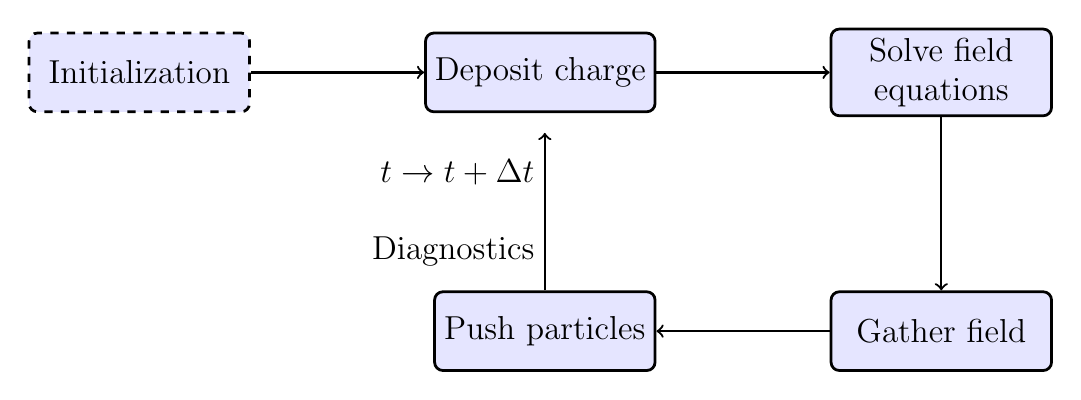
\begin{tikzpicture}[
    node distance=22mm,
    box/.style={
        draw,
        line width=1pt,
        rounded corners=3pt,
        fill=blue!10,
        minimum width=28mm,
        minimum height=10mm,
        align=center,
        font=\large,  
    },
    arrow/.style={->, thick},
]

% ----- Nodes: Horizontal layout -----
\node[box, dashed] (init) {Initialization};
\node[box, right=of init] (deposit) {Deposit charge};
\node[box, right=of deposit] (field) {Solve field\\equations};
\node[box,  below=of field] (gather) {Gather field};
\node[box, left=of gather] (push) {Push particles};


% ----- Arrows -----
\draw[arrow] (init) -- (deposit);
\draw[arrow] (deposit) -- (field);
\draw[arrow] (field) -- (gather);
\draw[arrow] (gather) -- (push);

% ----- Loop arrow from Diagnostics back to Deposit -----
\draw[arrow]
    (push.north) 
    -- ++(0,1)
        node[pos=0.5, left] {\large Diagnostics}
    -- ++(0,1)
        node[pos=0.5, left] {\large  $t\rightarrow t +\Delta t $ };
    % --  ++(0,0.2);
    % -- (deposit.south);
        

\end{tikzpicture}
\caption{Main loop of a Particle in Cell (PIC) simulation.}
\end{figure}


\subsubsection{Deposit charge}
To check the implementation of the charge deposition routine, we
designed a simple test with three macro-particles on a 1D grid of
length $L_x=1$ and $N_x=16$ cells.
The particle positions and charges are
\[
x_p = (0.10,\; 0.37,\; 0.92), \qquad
q_p = (-1.0,\; 0.5,\; -0.2),
\]
so that one particle lies close to the left boundary, one in the
interior of the domain, and one near the right boundary in order to
exercise the periodic wrapping.
The particles are deposited onto the grid using the CIC scheme,
producing a discrete charge density $\rho_i$.

As a consistency check, we compare the total charge carried by the
particles,
\[
Q_{\mathrm{part}} = \sum_p q_p,
\]
with the total charge obtained from the grid density,
\[
Q_{\mathrm{grid}} = \sum_i \rho_i \,\Delta x,
\]
where $\Delta x = L_x/N_x$.
In the code, both quantities are printed as
Sum of particle charges and Total deposited charge,
and their difference is found to be almost the same.
This confirms that the deposition algorithm conserves the total charge
exactly and behaves as expected for particles located near the
periodic boundaries.
\subsubsection{Poisson solver}

To verify the correctness of the implemented Poisson solver, we tested
it against several analytical benchmark cases under periodic boundary
conditions. The solver is designed to compute the electrostatic field
from the charge density by solving

\[
\frac{d^2\phi}{dx^2} = -\rho(x), \qquad E(x) = -\frac{d\phi}{dx}.
\]

\vspace{0.5em}
\noindent\textbf{Test cases:}


\textbf{Case 1:} $\rho(x)=0$.  
The numerical result gives $E \approx 0$ up to round--off level 
($\max|E|<10^{-15}$), confirming the solver preserves the trivial solution.

\medskip

\textbf{Case 2:} $\rho(x)=\cos(kx)$.  
The analytical solution is 
\[
\phi_{\text{ana}}(x)=\frac{\cos(kx)}{k^2}, \qquad 
E_{\text{ana}}(x)=\frac{1}{k}\sin(kx).
\]
Numerical results show $L_2$ error below $10^{-6}$ for $k=1,3$, 
indicating excellent agreement with theory.

\medskip

\textbf{Case 3:} high--wavenumber mode ($k=10$).  
The solver remains accurate with similarly small $L_2$ error,
demonstrating robustness for short--wavelength components.

\medskip

\textbf{Case 4:} random $\rho(x)$.  
The field computed by our solver matches the FFT--reconstructed
analytical reference with very small $L_2$ discrepancy.

\vspace{0.5em}
 
Across all tests, the numerical solutions overlap with the analytical
results almost perfectly, and the measured $L_2$ errors are on the
order of $10^{-6}$ to $10^{-10}$.  
This confirms that our Poisson solver is accurate and consistent
with theoretical predictions, and is therefore reliable for subsequent
PIC simulations.


\subsubsection{Gather field}
The field gather routine interpolates grid-based quantities back to
the particle positions.
We again use a CIC scheme, consistent with the
charge deposition step.
For a particle at position $x_p$, we locate the indices of the two
nearest grid points and compute the fractional coordinate inside the
cell.
The electric field at the particle is then obtained as a linear
combination of the surrounding grid values.

In continuous notation, the field at a particle can be written as
\[
  F_p = \sum_i F_i S(x_i - x_p),
\]
where $F_i$ is the grid field, $x_i$ is the position of grid point
$i$, and $S$ is the same linear shape function used for deposition.
In the code this reduces to
\[
  F_p = w_L F_{i_L} + w_R F_{i_R},
\]
with $w_L = 1-\xi$ and $w_R = \xi$ the CIC weights determined by the
particle position inside the cell.
Using the same shape function for both deposition and gathering
ensures that the PIC scheme is self-consistent.


\subsubsection{Push particle}
\subsubsection*{Boris algorithm}
Particle motion is evaluated using the standard Boris algorithm in a
leapfrog time discretization.

The Boris integrator exhibits excellent long-term stability when advancing 
charged particle trajectories. Owing to its leapfrog structure, the method 
introduces extremely small numerical energy drift even over millions of time 
steps. This makes the Boris scheme particularly well suited for PIC simulations 
in which particles must be evolved for long physical durations without artificial 
damping or secular energy growth.

A key geometric property of the Boris scheme is that it preserves the phase space 
volume of the particle trajectories,
\[
\det\!\left( \frac{\partial z^{\,n+1}}{\partial z^{\,n}} \right) = 1,
\qquad z = (\mathbf{x}, \mathbf{v}),
\]
ensuring that the algorithm does not introduce artificial compression or expansion 
of particle orbits. This volume-preserving (near-symplectic) nature prevents 
unphysical dissipation or numerical heating, and is crucial for accurately 
capturing Hamiltonian dynamics such as charged-particle motion in electromagnetic 
fields.

At each time step the code assumes that the particle positions
$x^n$ and the velocities $v^{n+1/2}$ are known.
The pusher first applies a half electric kick to obtain an
intermediate velocity,
\[
  \mathbf{u} = \mathbf{v}^{n+1/2} + \frac{q}{m}\mathbf{E}^n
  \frac{\Delta t}{2},
\]
then rotates $\mathbf{u}$ around the magnetic field using the
Boris rotation, and finally applies a second half electric kick
to obtain $\mathbf{v}^{n+3/2}$.
The new position is updated with the centered velocity,
\[
  x^{n+1} = x^n + v_x^{n+1/2}\Delta t,
\]
and periodic boundary conditions are enforced by wrapping the
position into the interval $[0,L_x)$.

In summary, by isolating and exactly resolving the magnetic field induced rotation, the Boris algorithm preserves kinetic energy and prevents numerical drift, giving it both higher accuracy and greater efficiency than widely used integrators such as forth order Runge-Kutta (RK4).

\subsubsection*{Validation of push particle}

To verify the implementation of the Boris pusher in our 1D3V code,
we consider a spatially uniform but time–oscillating electric field
and no magnetic field,
\[
E_x(t) = E_0 \sin(\omega t), \qquad B = 0 ,
\]
with the normalized charge–to–mass ratio $q/m=-1$.
The equation of motion then reads
\[
\frac{dv_x}{dt} = \frac{q}{m} E_x(t) = - E_0 \sin(\omega t).
\]
Integrating from $t=0$ with initial velocity $v_x(0)=v_0$ gives
\[
v_x(t) = v_0 + \frac{E_0}{\omega}\bigl(\cos(\omega t) - 1\bigr),
\]
and a second integration for the position (with $x(0)=x_0$) yields
\[
x(t) = x_0 + \left(v_0 - \frac{E_0}{\omega}\right)t
       + \frac{E_0}{\omega^2}\sin(\omega t).
\]

In the code, we evolve a single particle under this electric field
using the Boris pusher and record the numerical velocity
$v_{\mathrm{num}}(t_n)$ and position $x_{\mathrm{num}}(t_n)$ at each
time step.
These are compared with the analytical expressions
$v_{\mathrm{ana}}(t_n)$ and $x_{\mathrm{ana}}(t_n)$ above.
As shown in Fig.1, the numerical and analytical
curves for both $v_x(t)$ and $x(t)$ are almost indistinguishable;
the Boris pusher accurately reproduces the exact solution for this
time–dependent electric field.
\begin{figure}[h]
    \centering
    \includegraphics[width=0.70\textwidth]{test_push.png} 
    \caption{Numerical validation of the Boris pusher under an oscillating electric field}
    \label{fig:boris_E} 
\end{figure}



\subsection{Simulation setup}
To ensure that the results obtained from the PIC simulation are physically reliable a systematic convergence study is required.
In this work, we examine the sensitivity of the simulation outputs to variations in the key numerical parameters.
When one parameter is varied, the remaining parameters are consistent with those in \cref{tab:sim_params}.

\begin{table}[h]
\centering
\begin{tabular}{c|c|c}
\hline
Parameter & Value & Note \\
\hline
$L_x$ & 30 $\lambda_D$ & domain length \\
$Nx$ & $64$ & grid point \\
$Np$ & $5\times 10^5$ & total particles \\
$dt$ & 0.02 & time step \\
% steps & 1000 & total steps \\
$v_0$ & 1.0 & beam drift speed \\
$v_{th}$ & 0.1 & electron thermal speed \\
$n_0$ & $1\times10^{15}$ m$^{-3}$ & beam density per stream \\
\hline
\end{tabular}
\caption{Simulation parameters used in the PIC runs.}
\label{tab:sim_params}
\end{table}

\subsubsection{Spatial}
The periodic condition of fourier expansion gives $e^{ikL_x}=1$, which means $k_m=2\pi m /L_x\ (m= 1, 2, ..., N_x/2)$. From sec.2, one knows the wave number corresponding to the maximum grow rate: $k_{max}\approx0.86\ \lambda_D^{-1}\ (\hat{v}_0=1)$. 

Therefore, we choose $L=30$, which means the mode with $m=4$ nearly exactly matches the dominant unstable wavenumber. 
Also, there would be 4 phase space hole, i.e., BGK structure.

To assess spatial convergence, we vary the number of grid points $N_x = 16, 64, 128$, while holding all physical parameters constant, and examine the resulting changes in the growth rate and field structures. 
We have summarized the results under different spatial resolutions $N_x$ 
in a table, together with the corresponding phase space distributions shown below.
These figures illustrate how the system evolves as $N_x$ increases.


\begin{table}[h]
\centering
\begin{tabular}{c|c|c}
\hline
$N_x$ & Measured $\gamma$ & Convergence behaviour \\
\hline
16  & 0.344   & under-resolved \\
64  & 0.4683  & near convergence \\
128 & 0.4698  & converged \\
\hline
\end{tabular}
\caption{Measured growth rate $\gamma$ for different spatial resolutions $N_x$.}
\label{tab:gamma_resolution}
\end{table}

\begin{figure}[htbp]
    \centering
    
    \begin{subfigure}{0.32\textwidth}
        \centering
        \includegraphics[width=\linewidth]{N=16.png}
        \caption{$N_x=16$}
        \label{fig:nx16}
    \end{subfigure}
    \hfill
    \begin{subfigure}{0.32\textwidth}
        \centering
        \includegraphics[width=\linewidth]{N=64.png}
        \caption{$N_x=64$}
        \label{fig:nx64}
    \end{subfigure}
    \hfill
    \begin{subfigure}{0.32\textwidth}
        \centering
        \includegraphics[width=\linewidth]{N=128.png}
        \caption{$N_x=128$}
        \label{fig:nx128}
    \end{subfigure}
    
    \caption{phase space plots under different grid resolutions $N_x$.}
    \label{fig:phase_resolution_compare}
\end{figure}
As the grid resolution increases, the computational cost grows rapidly. 
Therefore, we adopt $N_x=64$ as it provides sufficient accuracy while maintaining reasonable efficiency.



\subsubsection{Particle number}

Following the analysis in the previous section, we fix the grid resolution at 
$N_x=64$ and investigate the effect of the particle number $N_p$ on the measured 
growth rate. The corresponding results are listed in \cref{tab:growth_np}.
In this and the following parts, we continue to fix all the simulation parameters except the one under investigation. 

\begin{table}[H]
\centering
\begin{tabular}{c|c|c}
\hline
\multicolumn{3}{c}{\textbf{Growth rate vs particle number $N_p$}}\\
\hline
$N_p$ & Measured $\gamma$ & Convergence behaviour \\
\hline
$1\times10^5$   & 0.4321 & under-sampled \\
$5\times10^5$   & 0.4683 & near convergence \\
$1\times10^6$   & 0.4739 & converged \\
\hline
\end{tabular}
\caption{Simulation parameters and measured growth rate for different particle numbers}
\label{tab:growth_np}
\end{table}


\subsubsection{Time}
Similarly, we now fix the spatial resolution and particle number at 
$N_x=64$ and $N_p=5\times10^5$, and vary the time step $dt$ from 0.01 and 0.02 up to 0.1 
to study its influence on the growth rate. From the table, the variation of the growth rate can be clearly observed.
\begin{table}[h]
\centering

\begin{tabular}{c|c|c}

\hline
\multicolumn{3}{c}{\textbf{Growth rate vs time step $dt$}}\\
\hline
$dt$ & Measured $\gamma$ &  Comment \\
\hline
0.01 & 0.4785 & converged \\
0.02 & 0.4683 & converged \\
0.10 & 0.4770 & nearly converged but not smooth \\
\hline
\end{tabular}
\caption{Simulation parameters and growth rate under different time steps}
\label{tab:growth_dt}
\end{table}

\begin{figure}[H]
    \centering
    
    \begin{subfigure}{0.32\textwidth}
        \centering
        \includegraphics[width=\linewidth]{dt=0.1.png}
        \caption{$dt=0.1$}
        \label{fig:dt01}
    \end{subfigure}
    \hfill
    \begin{subfigure}{0.32\textwidth}
        \centering
        \includegraphics[width=\linewidth]{dt=0.02.png}
        \caption{$dt=0.02$}
        \label{fig:dt002}
    \end{subfigure}
    \hfill
    \begin{subfigure}{0.32\textwidth}
        \centering
        \includegraphics[width=\linewidth]{dt=0.01.png}
        \caption{$dt=0.01$}
        \label{fig:dt001}
    \end{subfigure}
    
    \caption{Electric field energy growth rate fitting under different time steps $dt$ when m = 4.}
    \label{fig:Growth_rate_compare}
\end{figure}
Although the table indicates that $\gamma \approx 0.49$ when $dt=0.1$, 
the growth curve shows strong numerical noise in the later stage, which can be seen from \cref{tab:growth_dt}, suggesting that 
the measurement may not be reliable. Therefore, we choose $dt=0.02$ as a 
more accurate and stable setting.


\subsection{Full validation of the simulation}
In the following, we validate the simulation by examining its correctness from both qualitative and quantitative perspectives.
\subsubsection{Qualitative}
Based on the convergence analysis above, we adopt the grid resolution, particle number, and time step 
of $N_x = 64$, $N_p = 5\times 10^{5}$, and $\Delta t = 0.02$ for all subsequent simulations, 
with other parameters specified in \cref{tab:sim_params}.

As shown in \cref{fig:nx64}, distinct phase space holes, which also known as BGK structures, as discussed in Sec.~3.3.1. 
For $\hat v_0 = 1$, the dispersion relation predicts a dominant mode at $m = 4$, which corresponds to the formation of four BGK structures. 
This matches the pattern observed in \cref{fig:nx64} exactly, confirming that the simulation produces the correct qualitative behavior.

\subsubsection{Quantitative}
The quantitative correctness of the simulation can be assessed by comparing the growth rate of the dominant mode with the theoretical prediction.

\begin{table}[h]
\centering
\begin{tabular}{c|c|c}
\hline
$m$ & Measured $\gamma$ & Theoretical $\gamma$ \\
\hline
4 & $4.68 \times 10^{-1}$ & $5.00 \times 10^{-1}$ \\
3 & $4.32 \times 10^{-1}$ & $4.60 \times 10^{-1}$ \\
2 & $3.30 \times 10^{-1}$ & $3.50 \times 10^{-1}$ \\
\hline
\end{tabular}
\caption{Comparison of measured and theoretical growth rates $\gamma$ for different mode numbers $m$.}
\label{tab:gamma_m_compare}
\end{table}



The \Cref{fig:mode_growth} shows that all Fourier modes grow exponentially during the linear stage, with higher-order modes exhibiting faster growth. Mode 4 ($m=4$)
is the fastest-growing mode in our domain and becomes dominant before saturation.

The \Cref{fig:dispersion} presents the analytical cold-beam dispersion relation.
The theoretical growth rates for the corresponding wavenumbers ($m=4,\ 3,\ 2$) \footnote{The blue curve corresponding to $m=1$ represents a very weak mode whose linear growth stage is not observable. Therefore, it is omitted from the presented results.} matches very well with those measured from the PIC simulation. This agreement confirms that our PIC code successfully reproduces the linear instability physics.

\begin{figure}[h]
    \centering

    \begin{subfigure}{0.47\linewidth}
        \centering
        \includegraphics[width=\linewidth]{Pic1.png}
        \caption{Temporal evolution of electric field amplitudes}
        \label{fig:mode_growth}
    \end{subfigure}
    \hfill
    \begin{subfigure}{0.52\linewidth}
        \centering
        \includegraphics[width=\linewidth]{Pic2.png}
        \caption{Cold two stream instability dispersion relation}
        \label{fig:dispersion}
    \end{subfigure}

    \caption{Mode growth in simulation (left) and corresponding theoretical dispersion relation (right).}
    \label{fig:combined_modes}
\end{figure}



\section{Results analysis}
In the following, we vary the thermal velocity to transition from the cold plasma limit to a finite temperature plasma, allowing us to elucidate the key physical mechanisms of the two stream instability, including the origin of the instability and its saturation process. We further vary the beam velocity to illustrate how different beam speeds modify the mode structure. These results demonstrate the capability of our PIC simulations to capture and analyze the underlying physics.

\subsection{From cold plasma to finite temperature plasma——See how the wave particle resonance works}

In this part, we computed the growth rate $\gamma$ from the electric field energy 
evolution for each case, and plotted $\gamma$ as a function of $v_{\mathrm{th}}/v_0$. 
The curve exhibits a clear decreasing trend: the instability is strongest at low 
thermal velocity and is gradually suppressed as $v_{\mathrm{th}}$ increases, 
eventually approaching $\gamma \approx 0$ for sufficiently warm beams.


\begin{figure}[h]
    \centering
    \includegraphics[width=0.48\linewidth]{Growth rate.png}
    \caption{Growth rate $\gamma$ as a function of the thermal speed ratio $v_{\mathrm{th}}/v_0$.}
    \label{fig:growth_vth}
\end{figure}

As shown in \cref{fig:phase space distributions}, we analysed the system behaviour for different values of 
$v_{\mathrm{th}}$. The BGK structure in phase space clearly changes as the thermal 
velocity increases, indicating stronger phase space mixing and a reduction of 
coherent trapping structures.


\begin{figure}[H]
    \centering
    
    \begin{subfigure}{0.32\textwidth}
        \centering
        \includegraphics[width=\linewidth]{vth=0.1.png}
        \caption{$v_{{th}}=0.1$}
        \label{fig:vth01}
    \end{subfigure}
    \hfill
    \begin{subfigure}{0.32\textwidth}
        \centering
        \includegraphics[width=\linewidth]{vth=0.6.png}
        \caption{$v_{{th}}=0.6$}
        \label{fig:vth06}
    \end{subfigure}
    \hfill
    \begin{subfigure}{0.32\textwidth}
        \centering
        \includegraphics[width=\linewidth]{vth=1.png}
        \caption{$v_{{th}}=1.0$}
        \label{fig:vth1}
    \end{subfigure}
    
    \caption{phase space distributions for different thermal velocities $v_{{th}}$.}
    \label{fig:phase space distributions}
\end{figure}







This phenomenon originates from the physical mechanism of the two stream instability, which can be viewed as an extreme case of Landau wave particle resonance. An electrostatic wave exchanges energy with particles whose velocities are close to its phase velocity. When $\mathrm{d}f/\mathrm{d}v < 0$, more particles move slower than the wave and absorb energy from it, leading to damping. In contrast, if $\mathrm{d}f/\mathrm{d}v > 0$, particles transfer their kinetic energy to the wave, causing exponential growth.

For the two stream system, the velocity distribution contains a region with $\mathrm{d}f/\mathrm{d}v > 0$ (the interval between the two beams), as shown in \cref{fig:vth_01}. In this regime, resonant particles transfer kinetic energy to the field, leading to an exponential growth of the mode during the linear stage. 
As the system evolves, the wave amplitude increases and eventually becomes strong enough to trap resonant electrons inside its electrostatic potential wells as shown in the center of \cref{fig:two_stream_nonlinear} {Where we used $-\phi$ to represent the electrostatic potential energy of a electron.}. 
These trapped particles execute closed orbits in phase space, giving rise to the characteristic BGK type phase space holes. Through this trapping process, the distribution function is progressively reshaped around the phase velocity, the positive slope region $\mathrm{d}f/\mathrm{d}v > 0$ is flattened as shown in the bottom of \cref{fig:two_stream_nonlinear}, and the instability ultimately saturates once this region is effectively removed.


\begin{figure}[h]
    \centering

    % --- Left: Simulation at the beginning ---
    \begin{subfigure}{0.42\linewidth}
        \centering
        \includegraphics[width=\linewidth]{two_stream_initial.png}
        \caption{At the beginning of the simulation.}
        \label{fig:two_stream_initial}
    \end{subfigure}
    \hspace{0.05\linewidth} % 控制两图间距,越小越近
    % --- Right: Nonlinear stage ---
    \begin{subfigure}{0.42\linewidth}
        \centering
        \includegraphics[width=\linewidth]{two_stream_nonlinear.png}
        \caption{Nonlinear stage.}
        \label{fig:two_stream_nonlinear}
    \end{subfigure}

    \caption{Comparison between the beginning of the simulation and the nonlinear stage of the phase space distribution, electrostatic potential energy and velocity distribution, respectively}
    \label{fig:two_stream_comparison}
\end{figure}


When the temperature increases, the two peaks of the distribution broaden and progressively fill the central region. This reduces the magnitude and extent of the $\mathrm{d}f/\mathrm{d}v > 0$ interval, weakening the instability. At sufficiently large temperature, the valley disappears entirely and the distribution becomes single-humped, at which point the instability is suppressed.
This result highlights an important advantage of PIC simulations over analytical theory, namely their ability to account for more general and realistic physical conditions.


\begin{figure}[H]
    \centering
    
    \begin{subfigure}{0.32\textwidth}
        \centering
        \includegraphics[width=\linewidth]{f_vth=0.1.png}
        \caption{$v_{\mathrm{th}} = 0.1$}
        \label{fig:vth_01}
    \end{subfigure}
    \hfill
    \begin{subfigure}{0.32\textwidth}
        \centering
        \includegraphics[width=\linewidth]{f_vth=0.6.png}
        \caption{$v_{\mathrm{th}} = 0.6$}
        \label{fig:vth_06}
    \end{subfigure}
    \hfill
    \begin{subfigure}{0.32\textwidth}
        \centering
        \includegraphics[width=\linewidth]{f_vth=1.0.png}
        \caption{$v_{\mathrm{th}} = 1.0$}
        \label{fig:vth_10}
    \end{subfigure}

    \caption{Velocity distribution functions $f(v)$ for different thermal velocities $v_{\mathrm{th}}$ in a two stream plasma. 
    Increasing $v_{\mathrm{th}}$ broadens each Maxwellian beam and reduces the depth of the central gap between the two streams.}
    \label{fig:f_vth}
\end{figure}



\subsection{Different $v_0$ scan}
We also compared the growth rates for different beam velocities $v_0$, as shown in \cref{tab:growth_v01}. 
The variation of the growth rate with respect to $v_0$ is relatively small,as expected.

\begin{table}[h]
\centering

\begin{tabular}{c|c|c|c}
\hline
$v_0$ & Measured $\gamma$ & Theoretical $\gamma$  & Dominant mode\\
\hline
1 & $4.68\times 10^{-1}$ & $5.00\times 10^{-1}$  & $m=4$\\
2 & $4.75\times 10^{-1}$ & $5.00\times 10^{-1}$  & $m=2$\\
3 & $4.52\times 10^{-1}$ & $4.60\times 10^{-1}$  & $m=1$\\
\hline
\end{tabular}
\caption{Measured and theoretical growth rate $\gamma$ comparison for different beam speeds $v_0$.}
\label{tab:growth_v01}
\end{table}

From the phase space plots, we also observe that different values of $v_0$ lead to distinct BGK structures. 
Although the growth rates remain similar, the qualitative shape of the phase space vortices changes with $v_0$. These phase space results are consistent with our prediction in Section 3.3.1, where the number and shape of the BGK structures were shown to depend on the beam velocity $v_0$. The simulations clearly reproduce the expected variation in the number of trapped-particle islands, confirming the theoretical analysis.

\begin{figure}[H]
    \centering
    
    \begin{subfigure}{0.32\textwidth}
        \centering
        \includegraphics[width=\linewidth]{v0=1.png}
        \caption{$v_0 = 1.0$}
        \label{fig:v0_1}
    \end{subfigure}
    \hfill
    \begin{subfigure}{0.32\textwidth}
        \centering
        \includegraphics[width=\linewidth]{v0=2.png}
        \caption{$v_0 = 2.0$}
        \label{fig:v0_2}
    \end{subfigure}
    \hfill
    \begin{subfigure}{0.32\textwidth}
        \centering
        \includegraphics[width=\linewidth]{v0=3.png}
        \caption{$v_0 = 3.0$}
        \label{fig:v0_3}
    \end{subfigure}

    \caption{phase space distributions for different beam velocities $v_0$.}
    \label{fig:phase_v0}
\end{figure}

\section{Discuss and Conclusion}

In this work, we developed a modular 1D3V electrostatic PIC code capable of simulating the classical two stream instability.  
By comparing the numerical results with theoretical predictions, we validated both the accuracy of each individual module and the correctness of the integrated system.  
These tests confirm that the implementation reliably captures the linear growth, nonlinear saturation, and phase space structures associated with the instability.

Furthermore, our simulations allowed us to examine how the system evolves from an initially cold configuration to a thermally broadened state, thereby revealing the key physical mechanisms underlying the two stream instability.  
We also investigated how different beam velocities influence the resulting unstable modes and phase space dynamics.  
These results demonstrate the advantages of PIC simulations over purely theoretical analyses.
 
Because the code is highly modular and includes several reserved interfaces for future extensions, it can be readily expanded to support higher-dimensional geometries and a broader range of physical conditions.  
This modularity ensures that the current implementation serves not only as a functional solver for the two stream instability but also as a flexible foundation for future PIC development.

\end{document}
